% Copyright 2009-2012 by Hermann_Elendner
%
% This is the official VGSF LaTeX beamer presentation style.
% Questions and suggestions to:  linux@wu.ac.at
%
% This file may be distributed and/or modified
% under the GNU Public License, version 3 or later.
%
% See the file docs/LICENSE for more details.
%
% $revision 797
%
%%%%%%%%%%%%%%%%%%%%%%%%%%%%%%%%%%%%%%%%%%%%%%%%%%%%%%%%%%%%
%%%%                                                     %%%
%%%%     SEE THE FILE docs/README.txt  FOR GUIDANCE      %%%
%%%%                                                     %%%
%%%%                                                     %%%
%%%%%%%%%%%%%%%%%%%%%%%%%%%%%%%%%%%%%%%%%%%%%%%%%%%%%%%%%%%%
%
\documentclass{beamer}

%% suggested default packages:
\usepackage[utf8]{inputenc} % encoding of the .tex file
\usepackage[T1]{fontenc}    % use vector font
\usepackage{textcomp}       % to get symbol textbullet
\usepackage{lmodern}        % pick font (newest CM-like)
\usepackage[round]{natbib}  % for citations: \citet, \citep
\usepackage{pstricks}       % for psfigure drawings


\usepackage{psfrag}
\usepackage{multirow}
\usepackage{tikz}
\usepackage{graphicx}
\usepackage{caption}
\usepackage{subfig}
\usepackage{amsmath}
\usetikzlibrary{arrows,shapes,trees}
\usepackage{color}

\usepackage{algorithmic}
\usepackage{algorithm2e}
\renewcommand{\algorithmicrequire}{\textbf{INPUT:}}
\renewcommand{\algorithmicensure}{\textbf{OUTPUT:}}
\renewcommand{\algorithmicforall}{\textbf{for each}}

%%%>>> please adjust META INFORMATION here: ············<<<%
                                                           %
\author{Rüdiger Frey and Juraj Hledík}                               %
                                                           %
%%\title[short title]{long verbose elaborate title}        %
\title[Correlation and Contagion]{Correlation and Contagion as Sources of Systemic Risk}            %
                                                           %
%% optionally, define where presented (or leave empty)     %
\newcommand{\occasion}{PhD Defense 2018}               %
                                                           %
%% please don't define \institute, it's already defined.   %
%%%>>>··················································<<<%


%%>> ====== PREAMBLE =======================================
%%                                                        %%
%%  put here everything you'd like to put in the preamble %%
%%  e.g., \usepackages, \newcommands, etc                 %%
%%                                                        %%

\def\R{\mathbb{R}} 						% mnozina realnych cisel
\def\N{\mathbb{N}} 						% mnozina prirodzenych cisel
\def\F{\mathbb{F}} 						% filtracia
\newcommand{\dif}[1]{\mathrm{d}#1} 	% kolme d pri integrovani
\newcommand{\E}[1]{\mathrm{E}#1} 	% Stredna hodnota
\newcommand{\Cov}[1]{\mathrm{Cov}#1}% Kovariancia
\newcommand{\Var}[1]{\mathrm{Var}#1}% Variancia
\newcommand{\Cbid}[1]{C_{BID}#1}% Bid cena opcie
\newcommand{\Cask}[1]{C_{ASK}#1}% Ask cena opcie




%%>> SWITCHES (set 'true' or 'false'): 
\newcommand{\excludeAppendix}{false} % ignore backup slides%
\newcommand{\includePartPages}{true} % parts' interim slide%

%%>> pleae do not change these three lines: ·············<<%
\usepackage{themes/beamerthemeVienna}    % load VGSF style %
\usepackage{themes/beamerouterthemeVGSF} % all 3 required  %
\usepackage{themes/beamercolorthemeVGSF} % right here      % 
%%>>·····················································<<%
%%
%%>> ====== BEGIN DOCUMENT =================================
\begin{document}
\tikzstyle{every picture}+=[remember picture]
\everymath{\displaystyle}
%>--- TITLE PAGE: -------------------------------------
\maketitle

%>-=- PART -=-=-=-=-=-=-=-=-=-=-=-=-=-=-=-=-=-=-=-=-=-=
%\begin{frame}
%\begin{figure}[ht]
%\centering
%		
\includegraphics[width=0.75\textwidth]{images/title}
%\end{figure}
%\end{frame}

%>--- Slide -------------------------------------------
\begin{frame}{Systemic Risk}
	\textit{In finance, systemic risk is the risk of collapse of an entire financial system or entire market, as opposed to risk associated with any one individual entity, group or component of a system, that can be contained therein without harming the entire system. [...] It refers to the risks imposed by interlinkages and interdependencies in a system or market, where the failure of a single entity or cluster of entities can cause a cascading failure, which could potentially bankrupt or bring down the entire system or market.}\\
	\hfill -Wikipedia
\end{frame}

\begin{frame}{Channels of Systemic Risk}
	\begin{itemize}
		\item \textbf{Correlated portfolios} - exposures to common risk factors.
		\item \textbf{Counterparty Risk} - balance sheet contagion, insolvency cascades. 
		\item \textbf{Illiquidity} - mistrust, "gridlock".
		\item \textbf{Procyclical Feedback Effects} - fire sales.
		\item \ldots
	\end{itemize}
		\textcolor{white}{\textit{"We study interaction between correlated portfolio positions and direct lending of financial institutions in terms of systemic risk."
			}}
\end{frame}

\begin{frame}{Channels of Systemic Risk}
	\begin{itemize}
		\item \textcolor{red}{\textbf{Correlated portfolios}} - exposures to common risk factors.
		\item \textcolor{red}{\textbf{Counterparty Risk}} - balance sheet contagion, insolvency cascades. 
		\item \textbf{Illiquidity} - mistrust, "gridlock".
		\item \textbf{Procyclical Feedback Effects} - fire sales.
		\item \ldots
	\end{itemize}
	\textcolor{red}{\textit{"We study interaction between correlated portfolio positions and direct lending of financial institutions in terms of systemic risk."
	}}
\end{frame}
%>--- Slide -------------------------------------------


\begin{frame}{Overview}
\begin{itemize}
	\item Literature
	\item Model Setup
	\item Results
	\item Conclusions
\end{itemize}
\end{frame}

\begin{frame}{Literature}
	\begin{itemize}
		\item \textbf{Network Literature:}
		\begin{itemize}
			\item Beginnings: Allen and Gale (2000), Eisenberg and Noe, Furfine
			\item Regulators: Elsinger et al. (2006) - Austria, Gai and Kapadia (2010) - UK, Lubloy - Hungary, Mistrulli - Italy, Degryse and Nguyen - Belgium, Upper and Worms - Germany etc.
			\item Academics: Hurd et al., Battiston et al., Rama Cont, Andrea Minca, Hamed Amini and many others
		\end{itemize}
		\item \textbf{Literature on Dependent Defaults and Diversification}:
		\begin{itemize}
			\item Frey and McNeil (2003)
			\item Wagner (2010)
			\item Acharya and Yorulmazer (2007)
		\end{itemize}
	\end{itemize}
\end{frame}

\begin{frame}{Description of Financial Network}
\begin{itemize}
	\item We use graph theoretic concepts to characterize network of interbank relationships by modelling it as a graph $\mathbb{G}$.
	\item $\mathbb{G}$ is characterized by adjacency matrix $E$ with elements $e_{ij}$ satisfying:
	\begin{equation}
		\nonumber
		e_{ij}=\left\{ \begin{array}{cl}
			1 & \textrm{if $i$ is a debtor of $j$}\\
			0 & \textrm{if $i$ is not a debtor of $j$}
		\end{array}\right.
	\end{equation}
\end{itemize}
%\centering{\psfrag{A}{\textcolor{white}{Black Box}}
\includegraphics{images/BlackBox}}
\centering{$\downarrow$ Assumptions $\downarrow$}
\begin{figure}[ht]
	\centering
	\begin{tabular}{c||c}
		Assets & Liabilities \\ 
		\hline Interbank Assets $A_k^{IB}$  & Interbank Liabilities $L_k^{IB}$ \\ 
		External Assets $A_k^{EX}$ & External Liabilities $L_k^{EX}$ \\ 
		& Equity $\gamma$ \\
		\hline
		Total Assets $A_k$ & Total Liabilities $L_k$\\
	\end{tabular} 
	\caption{Balance sheet structure of bank $k$}
	\label{fig:TheModel:BalanceSheet}
\end{figure}
\end{frame}

\begin{frame}{2 Sources of Systemic Risk}
\begin{itemize}
	\item \textbf{Correlation:}
	\begin{itemize}
		\item If two banks $i,j$ invest in similar assets, their external assets $A^{EX}_i,A^{EX}_j$ face similar shocks.
		\item An extreme negative return towards their external portfolio can possibly cause their joint default.
	\end{itemize}
	\item \textbf{Contagion:}
	\begin{itemize}
	\item If a bank defaults, it can cause problems for its creditors and induce further insolvencies in a \textit{default cascade}.
	\end{itemize}
\end{itemize}
\end{frame}

\begin{frame}{2 Sources of Systemic Risk}
	\begin{itemize}
		\item \textcolor{red}{\textbf{Correlation:}}
		\begin{itemize}
			\item If two banks $i,j$ invest in similar assets, their external assets $A^{EX}_i,A^{EX}_j$ face similar shocks.
			\item An extreme negative return towards their external portfolio can possibly cause their joint default.
		\end{itemize}
		\item \textbf{Contagion:}
		\begin{itemize}
			\item If a bank defaults, it can cause problems for its creditors and induce further insolvencies in a \textit{default cascade}.
		\end{itemize}
	\end{itemize}
\end{frame}

\begin{frame}{Random returns}
\begin{itemize}
	\item Instead of lowering the capital buffer of random bank to zero, we assume that the initial shock takes a form of a negative return $r_k$ towards every bank's $k$ external assets $A^{EX}_k$:
	\begin{equation}
		r_k = \mu + \sqrt{\beta} r_M + \sqrt{(1-\beta)} \epsilon_k \nonumber
	\end{equation}
	where $r_M$ is the market return, $\epsilon_k$ is the idiosyncratic return of bank $k$ and $\beta$ measures the closeness to market portfolio.
	\item For $\beta=0$, banks are not correlated in terms of their external assets whereas for $\beta=1$ they are perfectly correlated.
	\item Both $r_M$ and $\epsilon_k$ are normally distributed such that $r_k$ is independent of $\beta$.
	\item The return realization is reflected on the level of bank $k$'s capital buffer. If it is negative enough, it can wipe out the buffer completely and the bank defaults.
\end{itemize}
\end{frame}

\begin{frame}{Density for $\beta=0$}
\begin{figure}[ht]
	\centering
		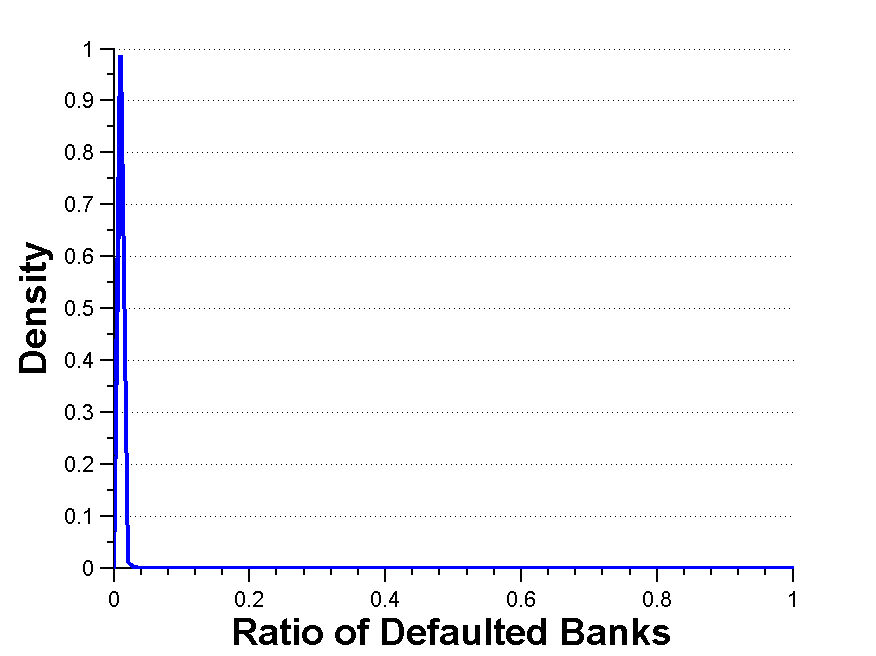
\includegraphics[width=0.7\textwidth]{images/ErdosRenyi_normal_beta_0_p_14}
	\caption{Ratio of defaulted banks over all banks in the system for $\beta=0$ (density function).}
	\label{fig:CreditRiskPicture}
\end{figure}
\end{frame}

\begin{frame}{2 Sources of Systemic Risk}
	\begin{itemize}
		\item \textbf{Correlation:}
		\begin{itemize}
			\item If two banks $i,j$ invest in similar assets, their external assets $A^{EX}_i,A^{EX}_j$ face similar shocks.
			\item An extreme negative return towards their external portfolio can possibly cause their joint default.
		\end{itemize}
		\item \textcolor{red}{\textbf{Contagion:}}
		\begin{itemize}
			\item If a bank defaults, it can cause problems for its creditors and induce further insolvencies in a \textit{default cascade}.
		\end{itemize}
	\end{itemize}
\end{frame}

\begin{frame}{Networks}
\begin{itemize}
	\item Contagion can induce further defaults.
	\item But how does the network look like?
	\item Regulator does not observe the network structure, usually only has partial information.
	\item There are some known stylized facts.
	\item If our network were a random variable, we could run a two-layer Monte Carlo simulation.
\end{itemize}
\end{frame}

\begin{frame}{Random Networks}
\begin{itemize}
	\item We generate a set of random networks according to two different algorithms.
	\item \textbf{Erdos-Renyi}:
	\begin{itemize}
	\item Any two banks in the system have the same probability $p_{ER}$ of being connected irrespective of the rest of the system.
	\end{itemize}
	\item \textbf{Core-periphery}:
	\begin{itemize}
	\item Each bank belongs to the core with probability $p_{core}$.
	\item Banks in core connect heavily with all banks in the system while peripherals only connect to other peripherals with very small probability.
	\end{itemize}
\end{itemize}
\end{frame}

\begin{frame}{Random Networks}
\begin{figure}[ht!]
	\centering
	\subfloat[Erdos-Renyi random graph]{
		\label{fig:Results:NetworkExamples:a} %% label for first subfigure
		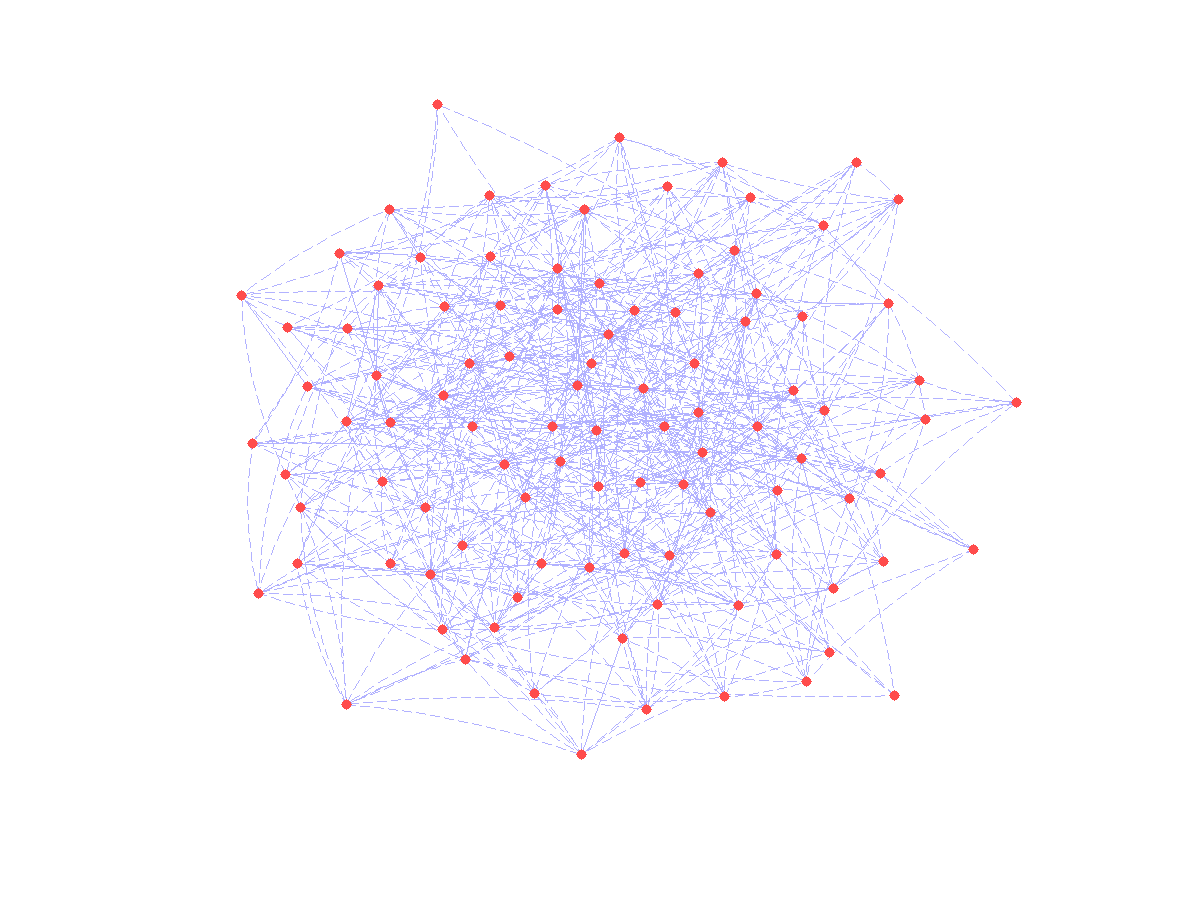
\includegraphics[width=0.45\linewidth]{images/ErdosRenyi}}
	\hspace{0.05\linewidth}
	\subfloat[Core-periphery random graph]{
		\label{fig:Results:NetworkExamples:b} %% label for first subfigure
		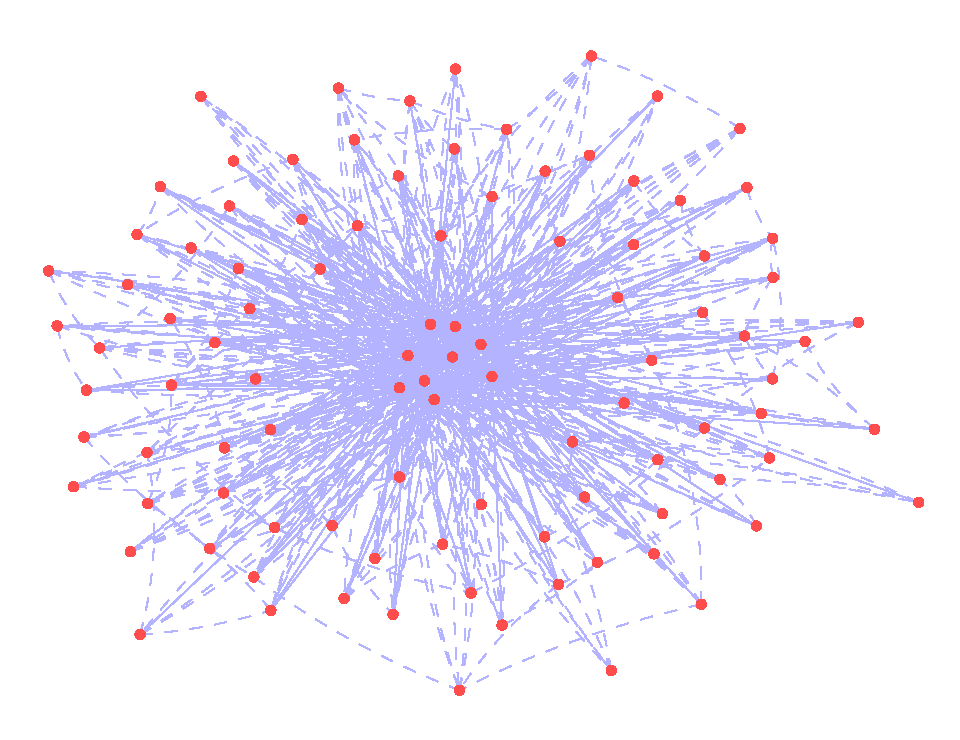
\includegraphics[width=0.45\linewidth]{images/Star}}
	\caption{Structural characteristics of networks. Both panels display a single realization of random graph for $N=100$ banks.}
	\label{fig:TheModel:NetworkExamples} %% label for entire figure
\end{figure}
\end{frame}

\begin{frame}{Density after contagion (for $\beta=0$)}
	\begin{figure}[ht]
		\centering
		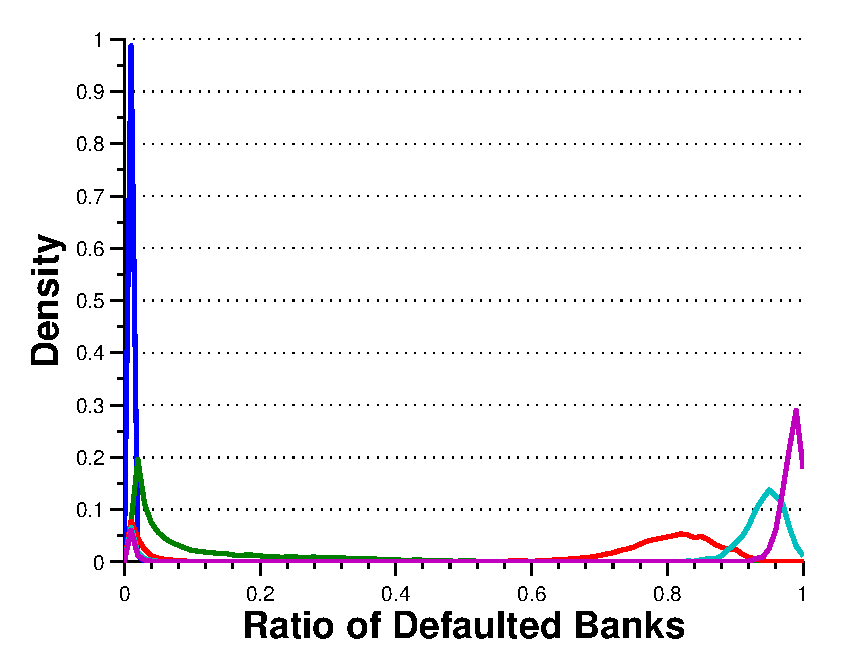
\includegraphics[width=0.6\textwidth]{images/all}
		\caption{Ratio of defaulted banks over all banks in the system for $\beta=0$ (density function after contagion). On average: \textcolor{blue}{Blue} = no network; \textcolor{green}{Green} = 1 neighbor; \textcolor{red}{Red} = 2 neighbors; \textcolor{cyan}{Cyan} = 3 neighbors; \textcolor{magenta}{Magenta} = 4 neighbors.}
	\end{figure}
\end{frame}

\begin{frame}{Results}
	\begin{figure}[!ht]
		\centering
		\psfrag{C}{\tiny{$C$}}
		\psfrag{beta=0xxxx}{\tiny{$\beta=0$}}
		\psfrag{beta=0.5xxxx}{\tiny{$\beta=0.5$}}
		\psfrag{beta=0.9xxxx}{\tiny{$\beta=0.9$}}
		\psfrag{Probability of Systemic Crisis}{\scriptsize{Probability of crisis}}
		\begin{tabular}{cc}
			\subfloat[Erdos-Renyi network]{
				\label{fig:Results:CutCorrelation:a} %% label for first subfigure
				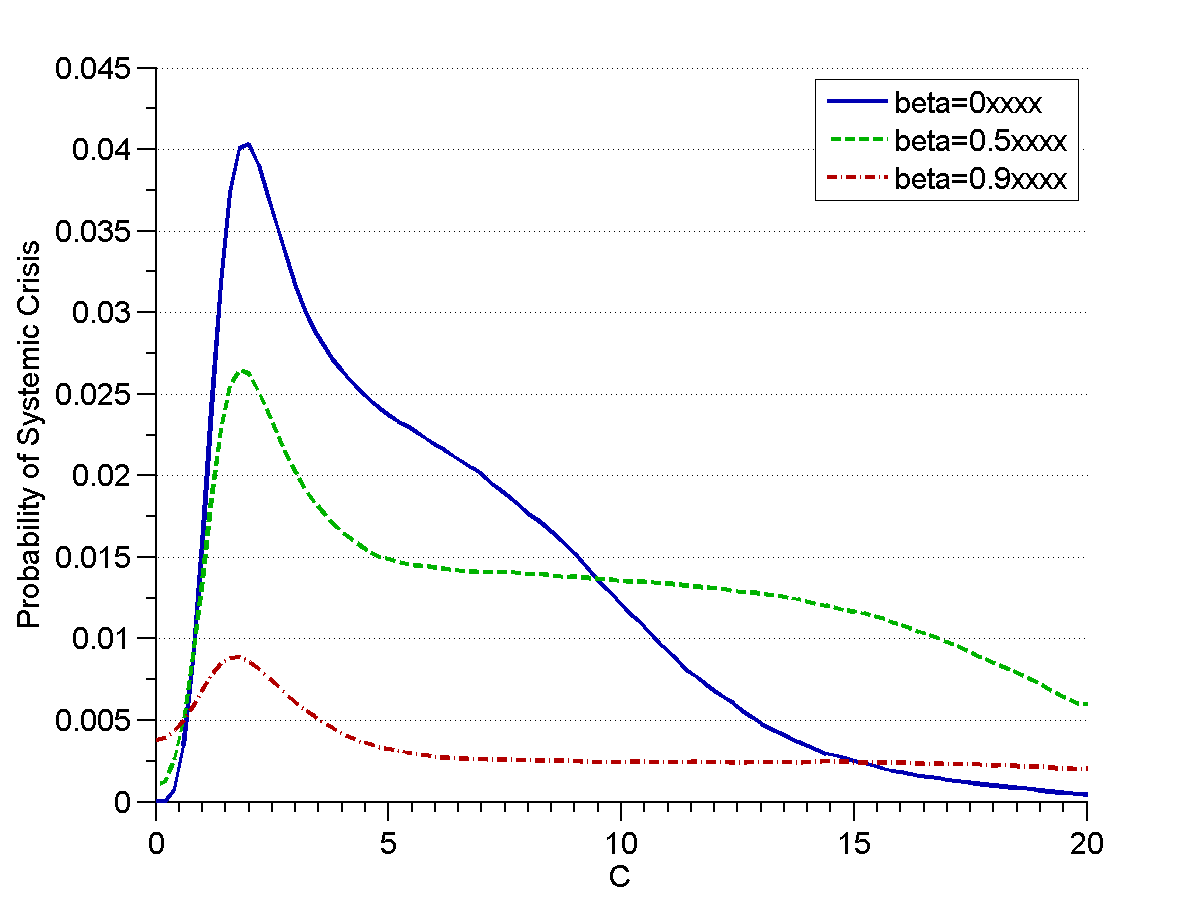
\includegraphics[width=0.42\linewidth]{images/ErdosRenyi/ErdosRenyi_normal_ScenFinalDefGivenThreshold_threshold02_CutCorrelation}}
			\hspace{0.05\linewidth}
			&
			\subfloat[Core-periphery network]{
				\label{fig:Results:CutCorrelation:b}
				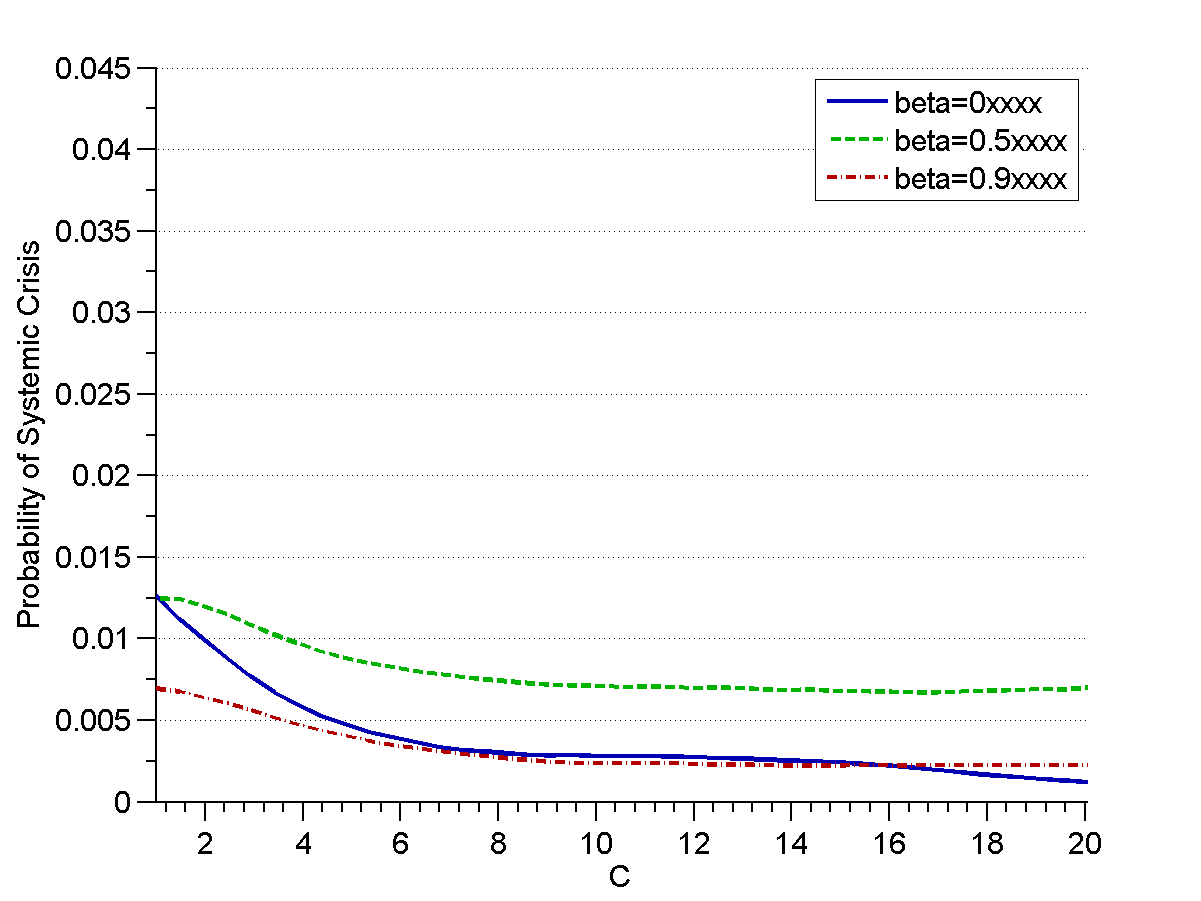
\includegraphics[width=0.42\linewidth]{images/Star/Star_normal_ScenFinalDefGivenThreshold_threshold02_both_kappa02_gamma0035_CutCorrelation}}
		\end{tabular}
		\caption{Share of scenarios with systemic crisis for both network structures on $N=100$ nodes as a function of network connectivity $C$ (average number of connections) for particular levels of correlation $\beta$.}
		\label{fig:Results:CutCorrelation} %% label for entire figure
	\end{figure}
\end{frame}



\begin{frame}{Results}
	\begin{figure}[!ht]
		\centering
		\psfrag{beta}{\tiny{$\beta$}}
		\psfrag{z=1xxxxxxx}{\tiny{$C=1$}}
		\psfrag{z=5xxxxxxx}{\tiny{$C=5$}}
		\psfrag{z=10xxxxxxx}{\tiny{$C=10$}}
		
		\psfrag{z=1xxxxxxx}{\tiny{$C=1$}}
		\psfrag{z=10xxxxxxx}{\tiny{$C=10$}}
		\psfrag{z=20xxxxxxx}{\tiny{$C=20$}}
		
		\psfrag{Probability of Systemic Crisis}{\scriptsize{Probability of crisis}}
		\begin{tabular}{cc}
			\subfloat[Erdos-Renyi network]{
				\label{fig:Results:CutConnectivity:a} %% label for first subfigure
				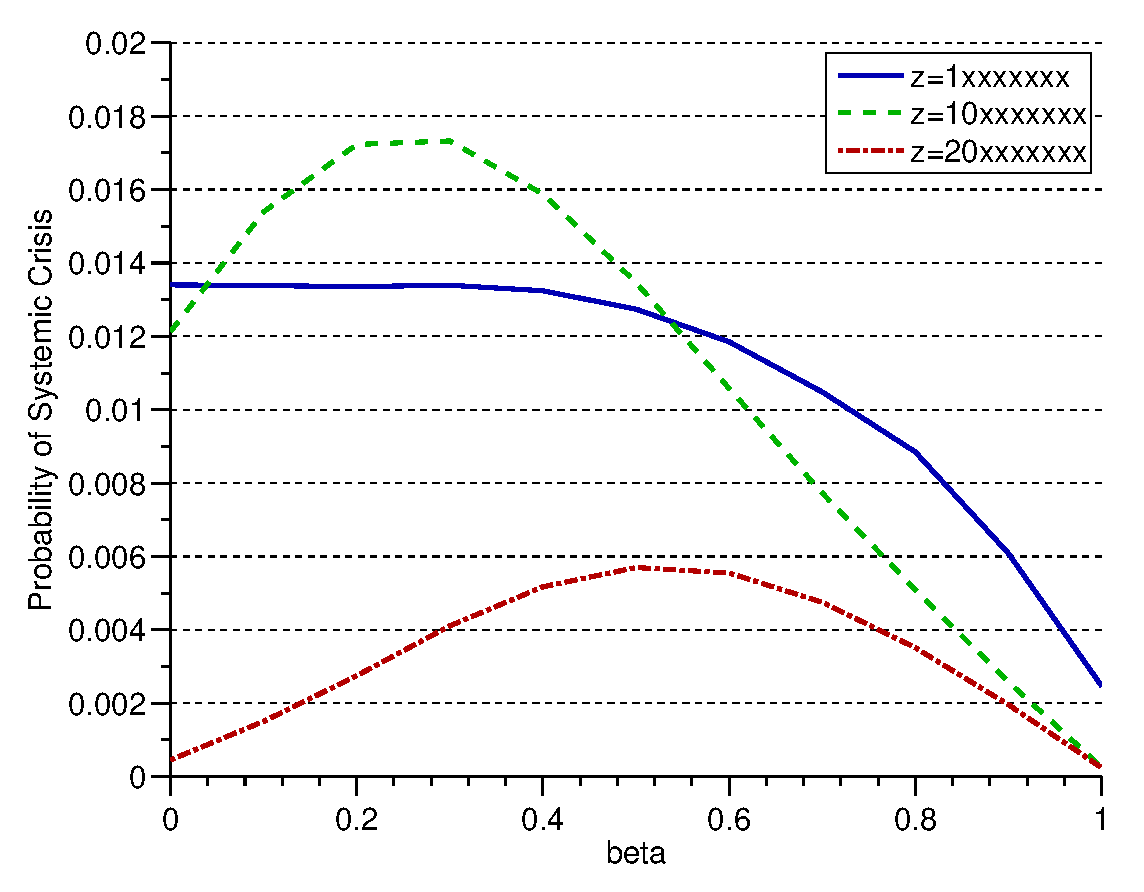
\includegraphics[width=0.42\linewidth]{images/ErdosRenyi/ErdosRenyi_normal_ScenFinalDefGivenThreshold_threshold02_CutConnectivity}}
			\hspace{0.05\linewidth}
			&
			\subfloat[Core-periphery network]{
				\label{fig:Results:CutConnectivity:b}
				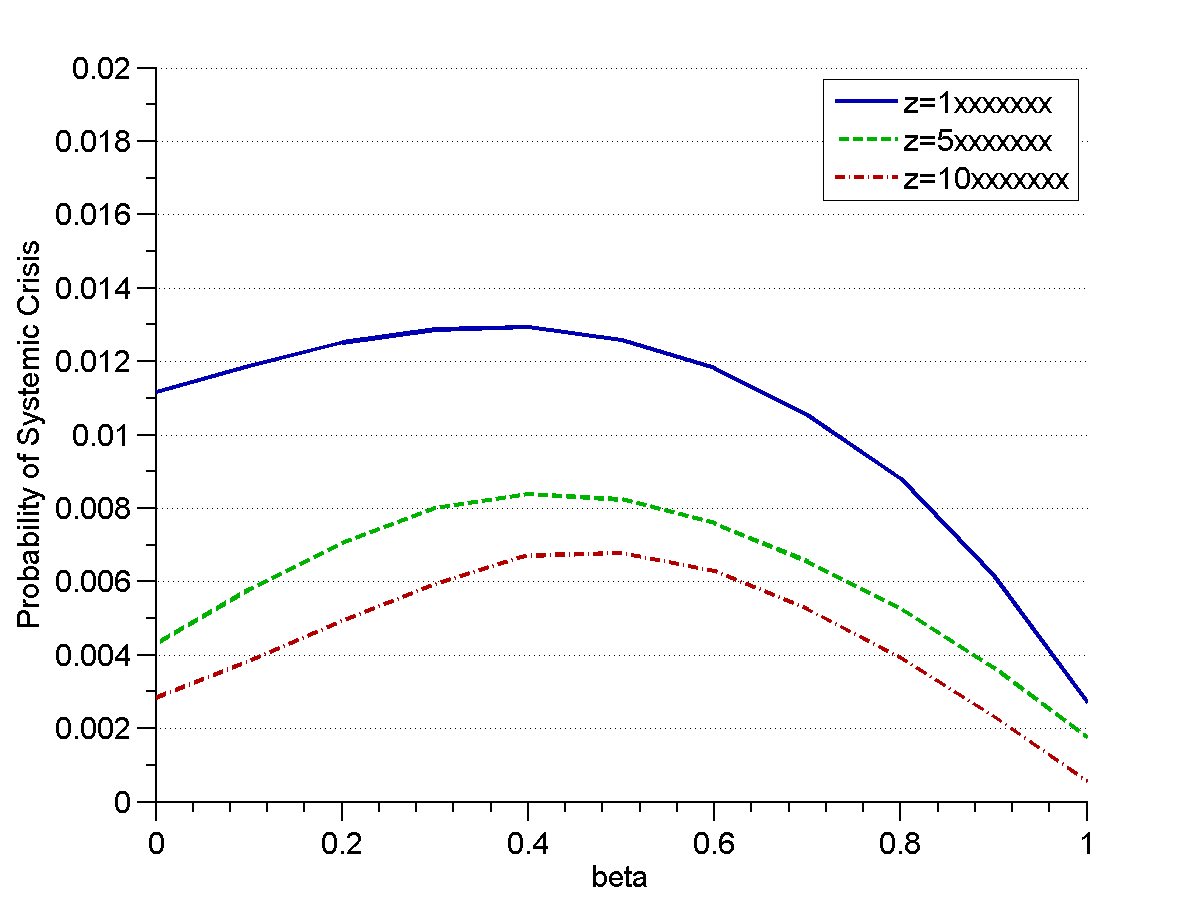
\includegraphics[width=0.42\linewidth]{images/Star/Star_normal_ScenFinalDefGivenThreshold_threshold02_both_kappa02_gamma0035_CutConnectivity}}
		\end{tabular}
		\caption{Share of scenarios with systemic crisis for both network structures on $N=100$ nodes as a function of correlation $\beta$ for particular levels of connectivity $C$ (average number of connections).}
		\label{fig:Results:CutConnectivity} %% label for entire figure
	\end{figure}
\end{frame}

\begin{frame}{Results and Conclusions}
\begin{itemize}
	\item \textbf{Results:}
	\begin{itemize}
		\item \textbf{No network} - Contagion cannot propagate. This is 	the case of Wagner (2010).
		\item \textbf{Some network} - If the network density is in a 	particular interval, increasing correlation is always beneficial. If it is more dense than this threshold, the effect of correlation is non-monotonous.
		\item \textbf{Dense network} - As we increase correlation between 	banks, systemic crises become more likely up to a certain threshold. Then the probability of a systemic event begins to decrease again.
	\end{itemize}
\end{itemize}
\end{frame}

\begin{frame}{Conclusions}
\begin{itemize}
	\item Interbank debt network structure and the level of correlation among external assets are tightly connected in terms of systemic risk.
	\item Core-periphery structure is more resilient than a homogeneous network.
	\item \textbf{Correlation is not always bad in terms of systemic risk.}
\end{itemize}
\end{frame}



%% >--- Bibliography ------------------------------------
% \begin{frame}[allowframebreaks]
%   \frametitle{Bibliography}
%   \footnotesize
%   \bibliographystyle{apalike} % OR {abbrvnat}
%   \bibliography{bib_literature}
% \end{frame}

%>= = BACKUP SLIDES = = = = = = = = = = = = = = = = = =
\begin{appendix}

%>--- Slide -------------------------------------------

%%>--- Slide -------------------------------------------
%\begin{frame}{You can make graphs like this with pstricks}
%   \begin{center}
%     %% You can easily produce graphs as follows with pstricks.  However, you
%     %% then need to compile .tex -> .ps -> .pdf (with latex), pstricks does
%     %% not work with pdflatex.  Therefore, the demo here is commented out;
%     %% just include the code and compile with latex to see how it works.
%     This slide shows a demo of how to draw graphs with \texttt{pstricks},
%     you just need to comment in the lines below this one in the .tex file.
%%     \begin{pspicture}(12,7)  % define max coordinates
%%       \psframe(0,0)(12,7)    % draw frame (at edges of coord system)
%%
%%       \rput[c](6,6.5){Note: this requires to compile with \LaTeX, not pdf\LaTeX!}
%%
%%       \psline[arrows=->](2,3)(5,4)  % draw line with arrow head
%%       \rput[r](2,3){given}          % put text, right-aligned
%%       \rput[l](5,4){gotten}         % put text, left-aligned
%%
%%       \psline[linestyle=dotted,arrows=|-|](1,6)(3,4)  % fancy line
%%       \rput{-45}(2,5.2){pstricks} % rotate -45°
%%
%%                               % works also within drawings
%%
%%       \psellipse[doubleline=true,linestyle=dashed,dash=4pt 2pt](9,3)(1.5,2.5)
%%       \rput[c](9,3){Columbus'}      % put text, centered
%%
%%       \rput(5,1.5){\pstribox[trimode=R,framesep=5pt]{\large\textbf{Begin}}}
%%
%%       %% MORE INFO ON HOW TO DRAW:  
%%       %% http://mirror.ctan.org/graphics/pstricks/base/doc/pstricks-doc.pdf
%%     \end{pspicture}
%   \end{center}
%\end{frame}




\begin{frame}{Results}
	\begin{figure}[!ht]
		\centering
		\psfrag{Probability of systemic crisis}{\tiny Probability of crisis}
		\psfrag{beta}{\tiny{$\beta$}}
		\psfrag{C}{\tiny{$C$}}
		\begin{tabular}{cc}
			\subfloat[Erdos-Renyi network]{
				\label{fig:Results:Surf:a} %% label for first subfigure
				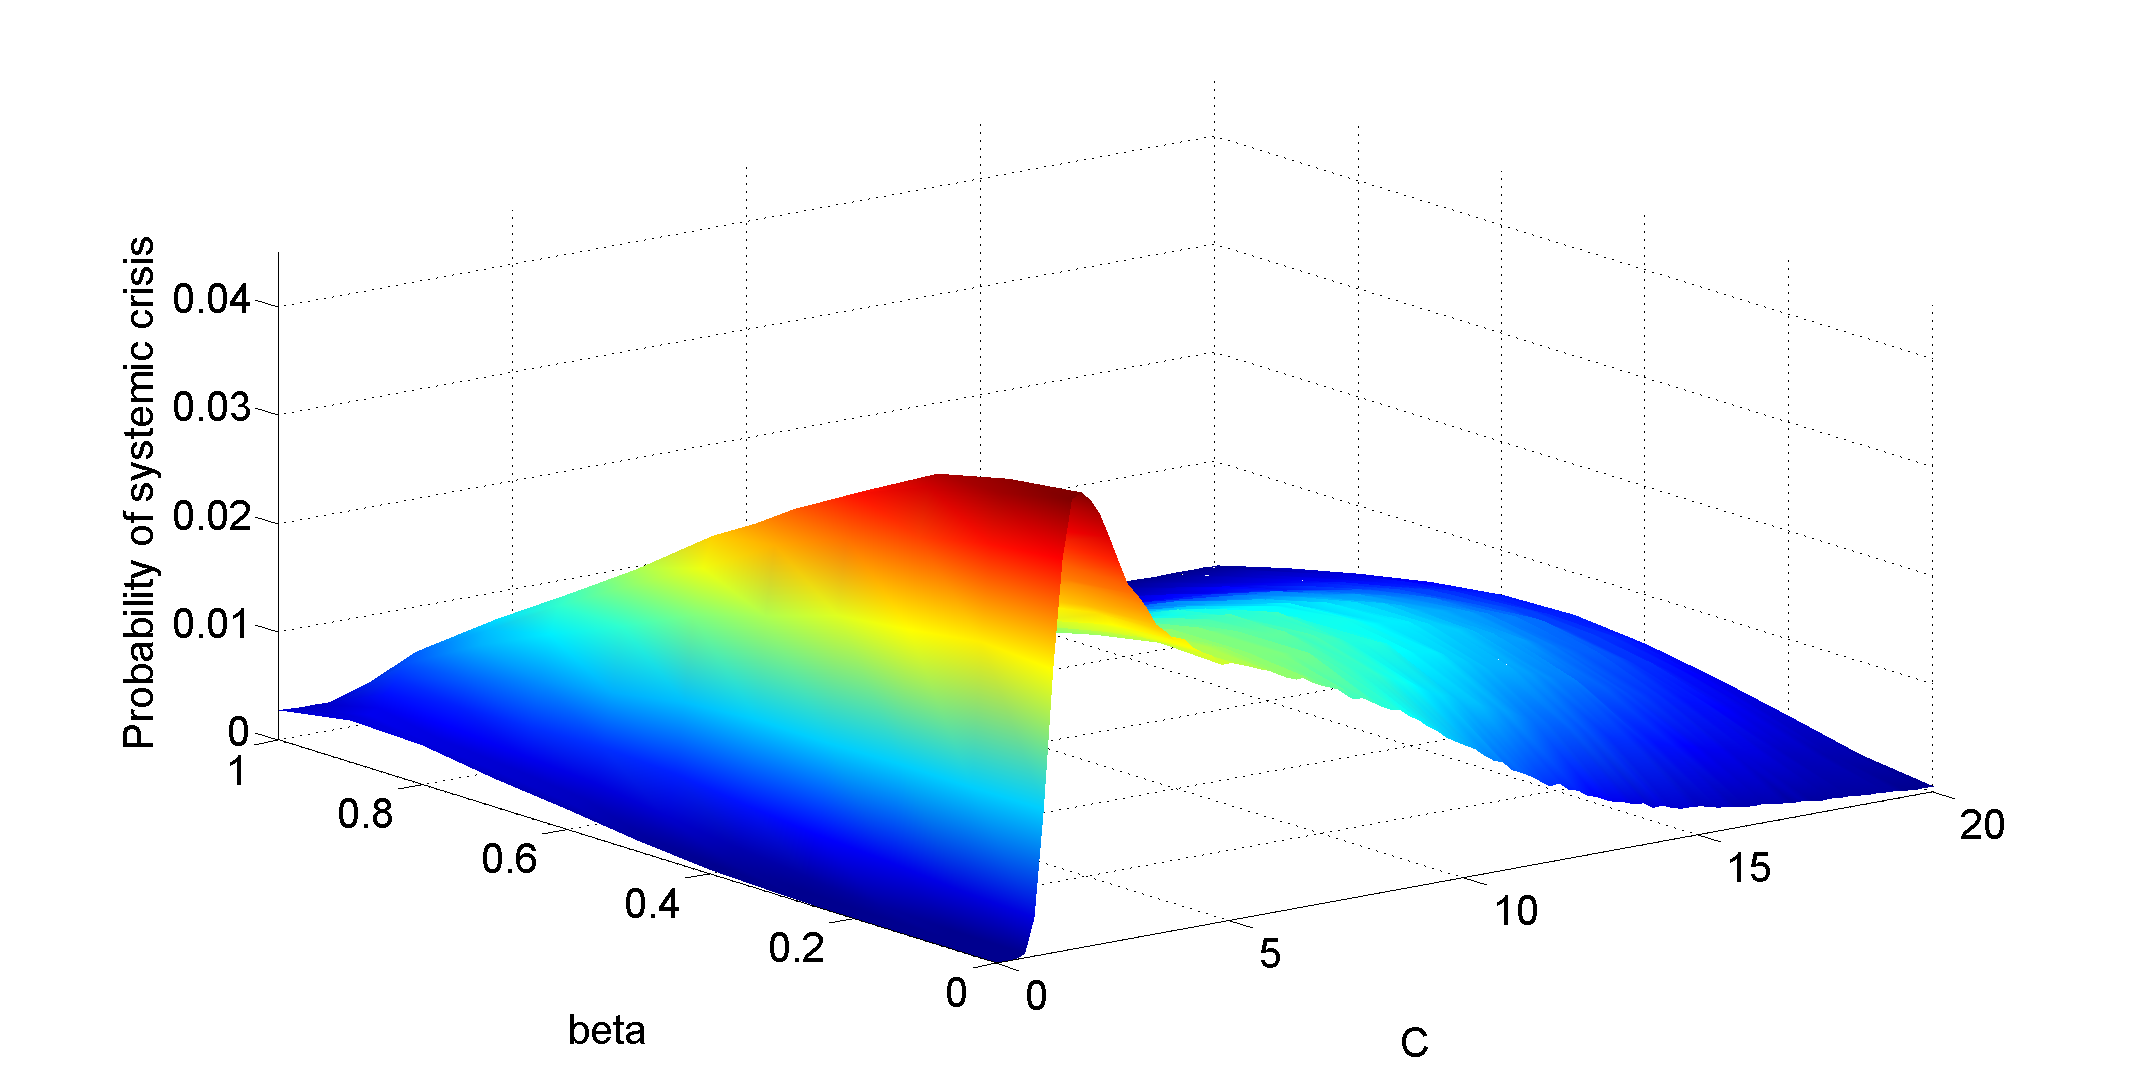
\includegraphics[width=0.42\linewidth]{images/ErdosRenyi/ErdosRenyi_normal_ScenFinalDefGivenThreshold_threshold02}
				\llap{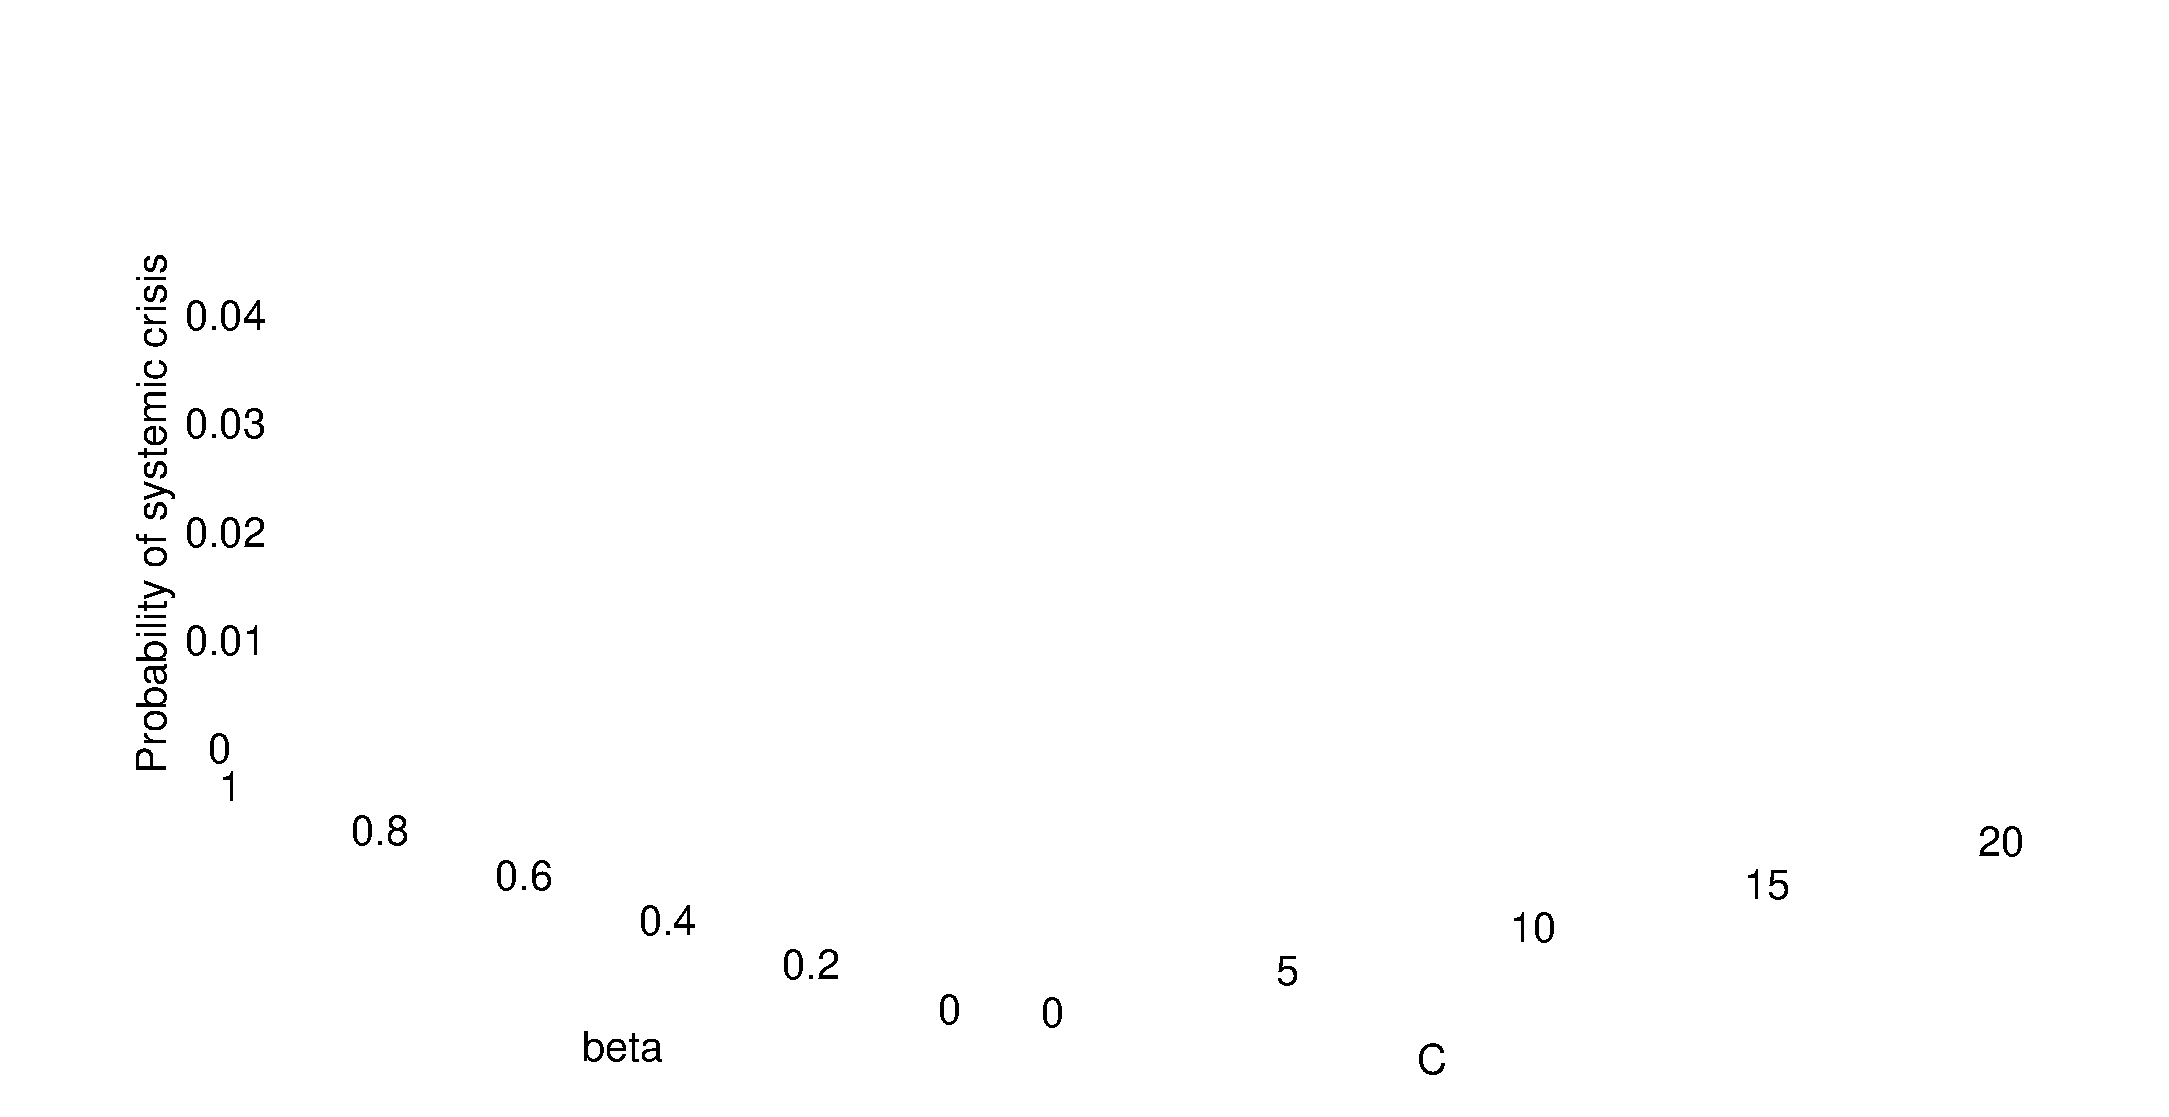
\includegraphics[width=0.42\linewidth]{images/ErdosRenyi/ErdosRenyi_normal_ScenFinalDefGivenThreshold_threshold02_t}
				}}
				\hspace{0.05\linewidth}
				&
				\subfloat[Core-periphery network]{
					\label{fig:Results:Surf:b}
					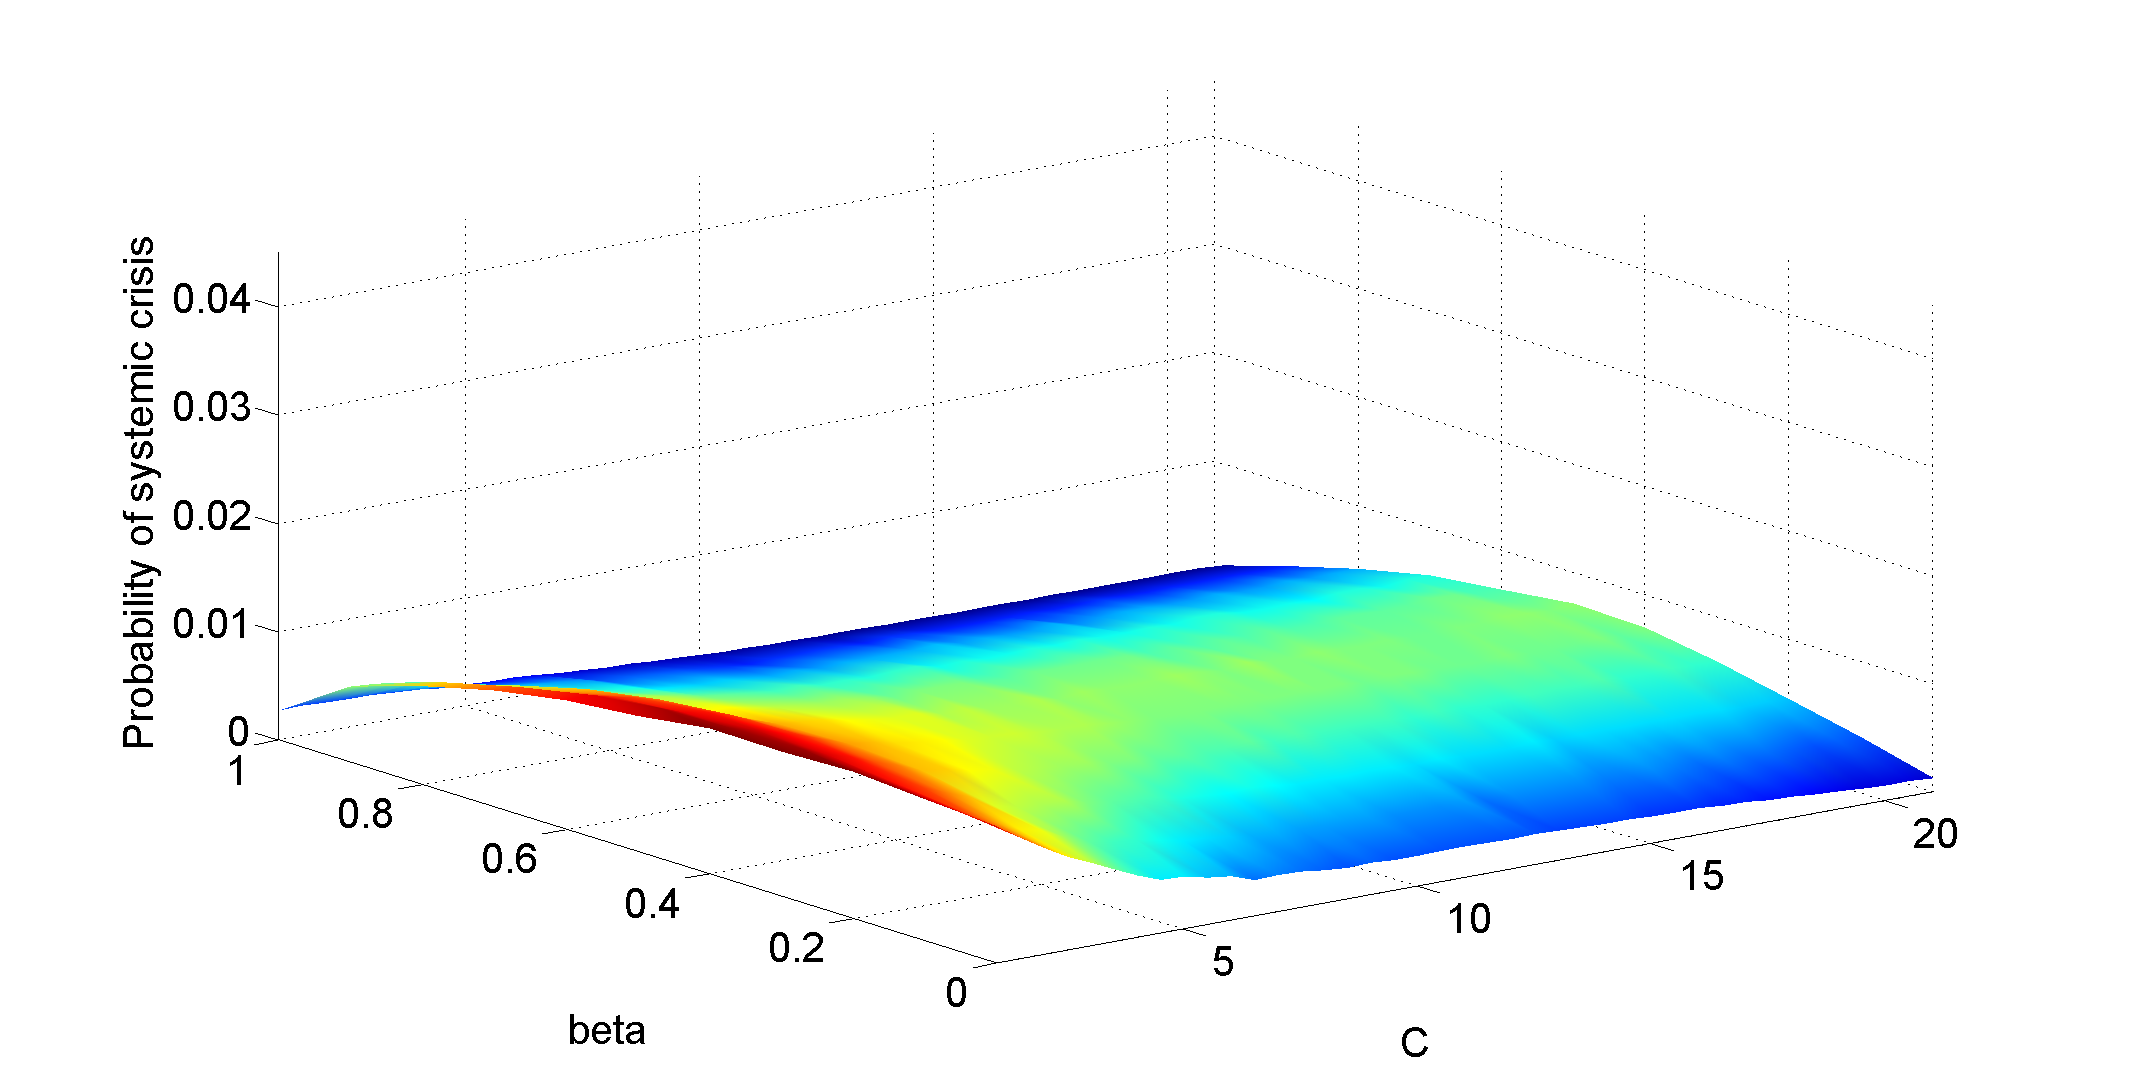
\includegraphics[width=0.42\linewidth]{images/Star/Star_normal_ScenFinalDefGivenThreshold_threshold02_both_kappa02_gamma0035}
					\llap{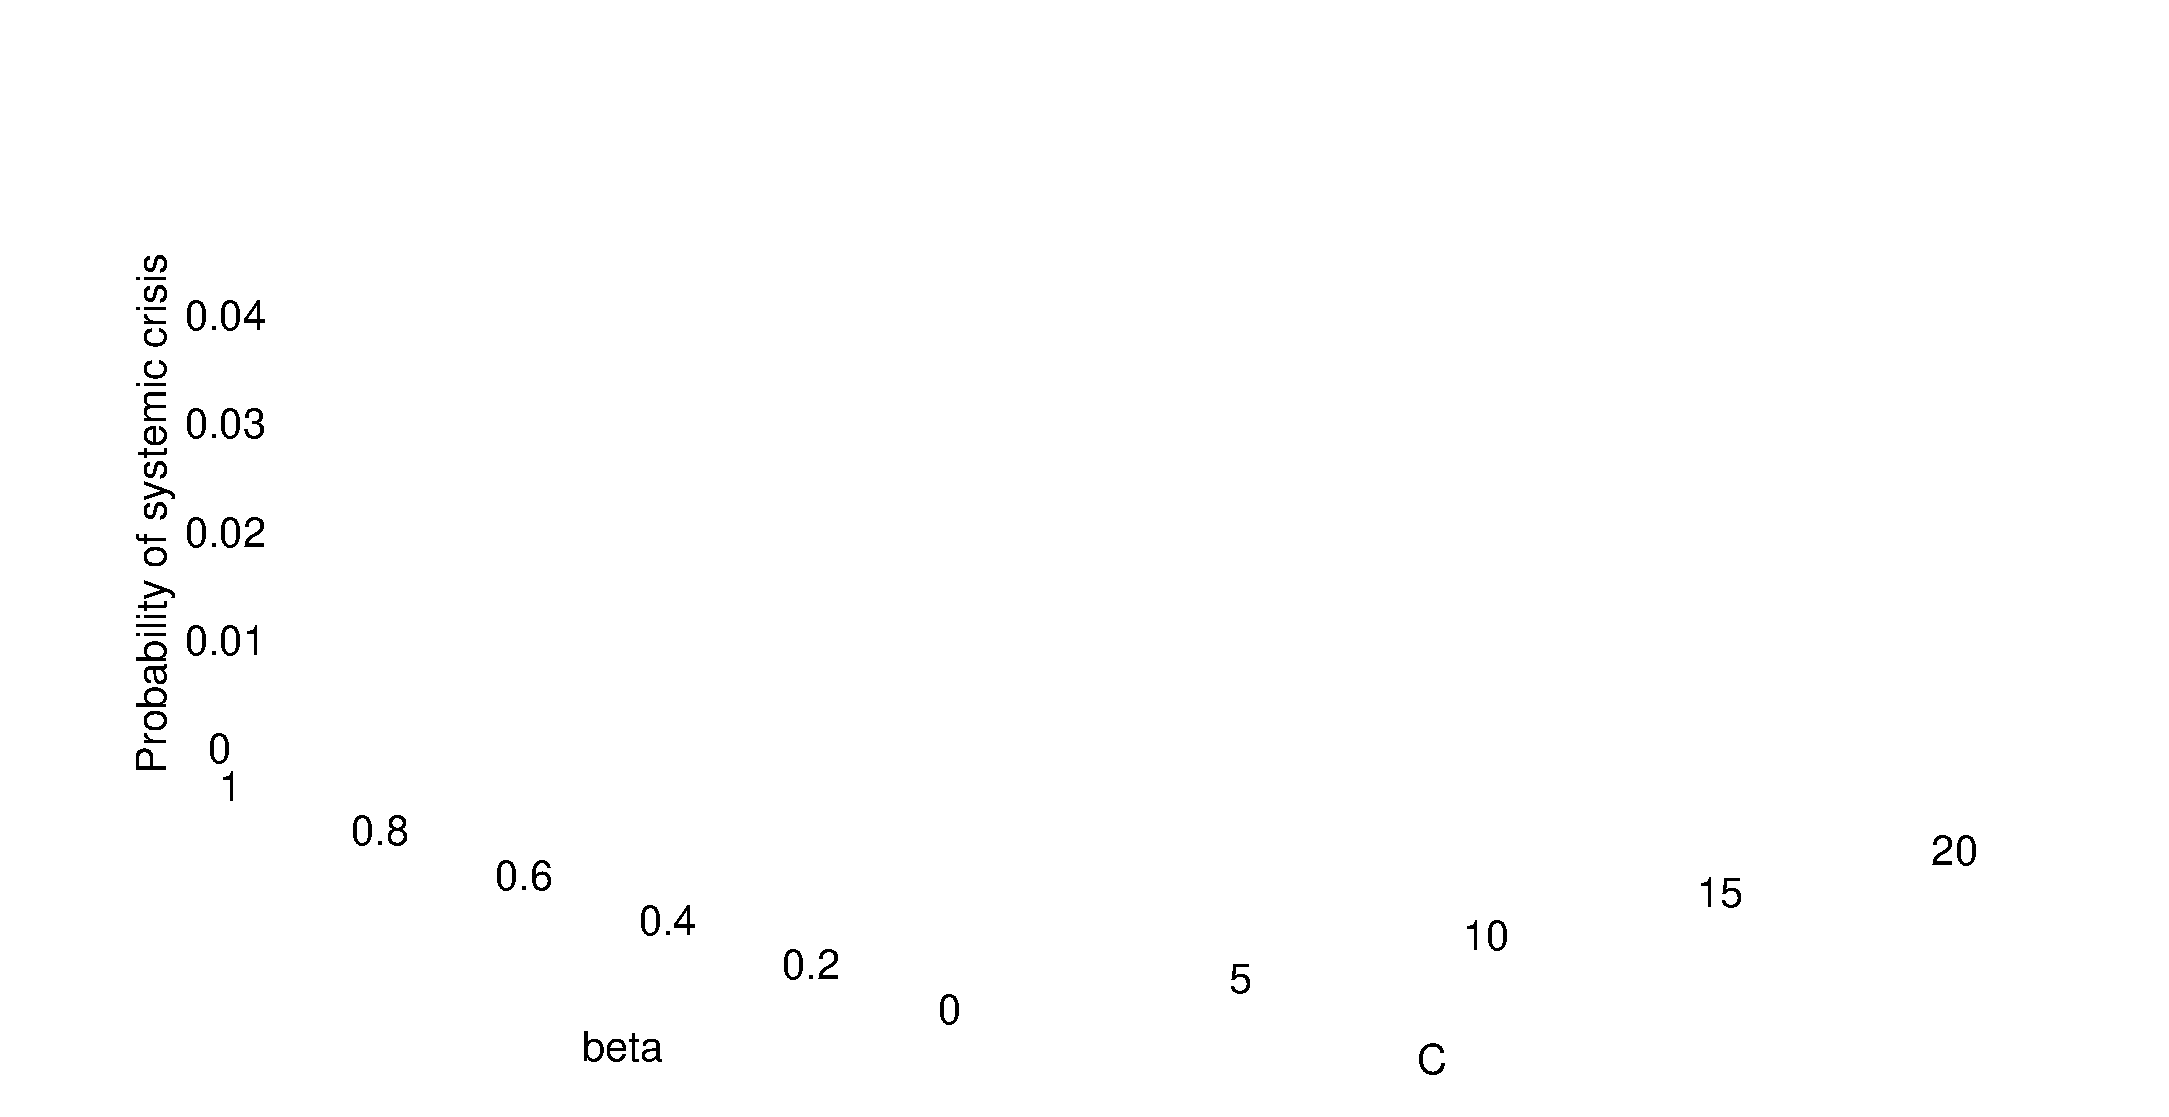
\includegraphics[width=0.42\linewidth]{images/Star/Star_normal_ScenFinalDefGivenThreshold_threshold02_both_kappa02_gamma0035_t}
					}}
		\end{tabular}
		\caption{Share of scenarios with systemic crisis for both network structures on $N=100$ nodes as a function of network connectivity $C$ (average number of connections) and level of correlation $\beta$.}
		\label{fig:Results:Surf} %% label for entire figure
	\end{figure}
\end{frame}
		

\begin{frame}{5 Steps of Balance Sheet Creation}
	\begin{enumerate}
		\item Take graph $\mathbb{G}$ on $N$ nodes characterized by matrix $E$.
		\item Determine sets of borrowers $I^B_k$ and lenders $I^L_k$ for every bank $k$.
		\item Assign the value of interbank assets $A^{IB}_k$ and liabilities $L^{IB}_k$ of every bank $k$ as
		\begin{equation}
		\nonumber
		A^{IB}_k:=|I^B_k| = \sum_{i} e_{ik} \ \ \ \ \ \ \ 		L^{IB}_k:=|I^L_k| = \sum_{j} e_{kj}
		\end{equation}
		\item Determine the total size of bank $k$'s balance sheet
		\begin{equation}
		\nonumber
		A_k=L_k:= \max\left[\frac{1}{\kappa}A^{IB}_k, \frac{1}{1-\gamma}L^{IB}_k\right]
		\end{equation}
		\item Set the external assets and external liabilities (deposits):
		\begin{equation}
		\nonumber
		A^{EX}_k:=A_k - A^{IB}_k \ \ \ \ \ \ \ 		L^{EX}_k:=(1-\gamma)L_k - L^{IB}_k
		\end{equation}
	\end{enumerate}
\end{frame}

\begin{frame}{Some Descriptives}
	\begin{table}
		\centering
		\begin{tabular}{l || c c}
			Return distribution	& Normal & Student \\
			\hline
			Individual default probability of a single bank (\%) & 0.024\% & 0.45\% \\
			Probability of at least one default ($\beta=0$) & 2.37\% & 23.42\% \\
			Probability of at least one default ($\beta=0.3$) & 1.97\% & 15.50\% \\
			Probability of at least one default ($\beta=0.5$) & 1.39\% & 10.69\% \\
			Probability of at least one default ($\beta=0.9$) & 0.25\% & 2.57\% \end{tabular}
		\caption{Descriptive statistics for both return distributions (N=100).}
		\label{tab:Results:DescriptiveStatistics}
	\end{table}
\end{frame}

\begin{frame}{Contagion Algorithm}
	\tiny{
	\begin{algorithmic}[1]
		\REQUIRE Adjacency matrix $E_\mathbb{G}$ with elements $e_{ij}$, balance sheet quantities $A^{IB}_k, A^{EX}_k, L^{IB}_k, L^{EX}_k, A_k, \gamma_k$ and the return realization of $r_k$ for every bank $k$.
		%
		\ENSURE Set of defaulted banks at the end of the cascade $I^{D}_T$.
		%
		\STATE $I^D_0:=\{\emptyset\}$;	\COMMENT{At time 0, every bank is safe}
		%
		\FORALL{$k\in \{1,2,\ldots,N\}$}
		%
		\STATE $\gamma_k:=\gamma_k + r_k\frac{A^{EX}_k}{A_k}$;	\COMMENT{Initial return shocks capital buffer and asset side.}
		%
		\STATE $A_k:=A_k + r_k A^{EX}_k$;
		%
		\STATE $A^{EX}_k:=(1+r_k)A^{EX}_k$;
		%
		\ENDFOR
		%
		\STATE $I^D_1:=\{k\in\{1,2,\ldots,N\},\gamma_k\leq 0\}$;	\COMMENT{Determine the set of time 1 defaulted banks.}
		%
		\STATE $t:=1$;
		%
		\WHILE{$I^D_t \not\equiv  I^D_{t-1}$}
		%
		\FORALL{$\{k: k\in I^{D}_t \wedge k\not\in I^D_{t-1}\}$}
		%
		\FORALL{$\{j: e_{kj}=1\}$}
		%
		\STATE $\gamma_j:=\gamma_j-\frac{1}{A_j}$ \COMMENT{Creditors $j$ of defaulted bank $k$ are shocked.}
		%
		\ENDFOR
		%
		\ENDFOR
		%
		\STATE $t:=t+1;$	\COMMENT{Next iteration.}
		%
		\STATE $I^D_{t}:=I^D_{t-1}$;
		%
		\FORALL{$k:k\not\in I^D_{t-1}$}
		%
		\IF{$\gamma_k\leq 0$}
		%
		\STATE $I^D_{t}:=I^D_{t} \cup \{k\}$;	\COMMENT{If $\gamma_k$ of $k$ falls below zero, mark it as in default.}
		%
		\ENDIF
		%
		\ENDFOR
		%
		\ENDWHILE
		%
		\STATE $I^D_T$=$I^D_t$;	\COMMENT{Final index set of defaulted banks.}
		%
	\end{algorithmic}
}
\end{frame}

\begin{frame}{Assumptions}
	\begin{enumerate}
		\item All loans in the system are of the same size, normalized to 1.
		\item The equity ratio of every bank $k$ is equal to an exogenously given constant $\gamma$.
		\item The level of integration $\kappa$ is fixed at the same value for each bank such that $A_k^{IB}=\kappa A_k$.
	\end{enumerate}
\end{frame}

\end{appendix}
\end{document}
%%>> ====== END DOCUMENT ===================================
%
% (c) hwe
%
%
% Room for notes: